\documentclass[12pt]{article}
\usepackage[utf8]{inputenc}
\usepackage[T1]{fontenc}
\usepackage{graphicx}
\usepackage{subcaption}
\usepackage{amsmath}
\usepackage{fancyhdr}
\usepackage{geometry}
\usepackage[english]{babel}
\usepackage{csquotes}
\usepackage{hyperref}
\usepackage{url}
\usepackage{listings}
\usepackage{float}
\usepackage{booktabs}
\usepackage{array}
\usepackage{tikz}
\usetikzlibrary{
    shapes.geometric, shapes.misc,
    arrows.meta, positioning, fit,
    backgrounds, calc, decorations.pathreplacing,
    automata
}
\usepackage{setspace}

\lstset{
    language=C,
    basicstyle=\ttfamily\small,
    numberstyle=\tiny,
    frame=single,
    breaklines=true,
}

% TikZ styles
\tikzset{
  comp/.style={rectangle, draw, rounded corners=3pt,
               minimum width=2.8cm, minimum height=0.75cm,
               align=center, font=\small},
  hw/.style={comp, fill=gray!20},
  driver/.style={comp, fill=blue!15},
  service/.style={comp, fill=green!15},
  task/.style={comp, fill=orange!20},
  app/.style={comp, fill=yellow!20},
  arr/.style={-Stealth, thick},
  biarr/.style={Stealth-Stealth, thick},
  layer/.style={rectangle, draw, minimum height=0.9cm,
                align=center, font=\small\bfseries},
  cls/.style={rectangle, draw, font=\small, text width=2.8cm,
              minimum width=3.0cm, inner sep=3pt},
  hdr/.style={cls, fill=gray!10, align=center, font=\small\bfseries},
  uses/.style={-Stealth, dashed, thick},
  impl/.style={-Stealth, thick},
  state/.style={circle, draw, fill=blue!10, minimum size=2.0cm,
                align=center, font=\small\bfseries},
}

\linespread{1.25}
\setlength{\parindent}{0.8cm}
\setlength{\parskip}{0em}
\renewcommand{\headrulewidth}{0pt}
\geometry{a4paper, portrait, margin=1in}
\setlength{\headheight}{14.49998pt}

\begin{document}
\begin{titlepage}
   \begin{center}
    \textsc{\large Ministry of Education of Republic of Moldova}\\[0.5cm]
    \textsc{\large Technical University of Moldova}\\[0.5cm]
    \textsc{\large Faculty of Computers, Informatics and Microelectronics}\\[0.5cm]
    \textsc{\large Software Engineering Department}\\[1.2cm]

    \vspace{25mm}

    {\LARGE \textbf{\textsc{Embedded Systems}}}\\[0.5cm]
    \textsc{\large Laboratory No. 1.8}\\[0.5cm]

    \newcommand{\HRule}{\rule{\linewidth}{0.5mm}}
    \vspace{80mm}

    \begin{minipage}[t]{0.4\textwidth}
    \begin{flushleft} \large
    \emph{Author:} \\
    Vladimir \textsc{Vitcovschii}\\
    std. gr. FAF-231
    \end{flushleft}
    \end{minipage}
    ~
    \begin{minipage}[t]{0.4\textwidth}
    \begin{flushright} \large
    \end{flushright}
    \end{minipage}\\[3cm]

    \vspace{5mm}
    \large Chi\c{s}in\u{a}u 2026\\[0.5cm]

    \vfill
    \end{center}
\end{titlepage}

\clearpage
\tableofcontents
\clearpage

\setcounter{page}{2}
\pagestyle{fancy}
\fancyhf{}
\rhead{\thepage}
\lhead{FAF-231 Vitcovschii Vladimir; Laboratory Work No. 1.8}

% ─────────────────────────────────────────────────────────────────────────────
\section{The Purpose of the Work}
% ─────────────────────────────────────────────────────────────────────────────

The purpose of this laboratory work is to upgrade the closed-loop temperature controller from Lab~1.7 by replacing the binary ON-OFF hysteresis law with a continuous \textbf{Proportional--Integral--Derivative (PID)} regulator. The plant and hardware remain unchanged: an NTC thermistor on A0 senses the process variable, and a servo motor on D9 acts as the actuator. The PID output is mapped to a continuous servo angle around a $90^{\circ}$ centre, providing fine-grained correction proportional to the magnitude of the regulation error. The work emphasises the implementation of a fixed-point PID step on a microcontroller without an FPU, anti-windup of the integral term, online tuning of the three gains via a serial command interface, and the visualisation of the closed-loop response with the Arduino Serial Plotter.

% ─────────────────────────────────────────────────────────────────────────────
\section{Objectives of the Work}
% ─────────────────────────────────────────────────────────────────────────────

The task requires implementing a complete PID temperature controller on an ATmega2560 with FreeRTOS, organised as five concurrent tasks plus a separate \texttt{PidController} module:
\begin{itemize}
  \item \textbf{Task~1 --- Acquisition (50\,ms)}: Read NTC, convert to tenths $^{\circ}$C, publish PV.
  \item \textbf{Task~2 --- CommandRead (50\,ms)}: Parse the serial line and the keypad. In addition to numeric set-point entry (digits + \texttt{\#}, \texttt{*} clear, \texttt{A}/\texttt{B}/\texttt{C}/\texttt{D} nudge), accept four runtime tuning commands: \texttt{P<float>}, \texttt{I<float>}, \texttt{D<float>}, and \texttt{RESET} (clear PID state).
  \item \textbf{Task~3 --- Control (100\,ms)}: Call \texttt{PidStep(SP, PV, Kp, Ki, Kd, \&I, \&E\_prev, IntegralLimit, OutputMax)}. Output is clamped to $[-100, +100]$.
  \item \textbf{Task~4 --- Actuator (50\,ms)}: Map the control output to a servo angle of $90^{\circ} + \mathrm{out}\cdot 90/100$, clipped to $[0, 180]^{\circ}$. Drive the green LED while $|\mathrm{err}| \le 1.0\,^{\circ}$C, the red LED on output saturation, and toggle the yellow heartbeat LED.
  \item \textbf{Task~5 --- Display (500\,ms)}: Emit a Plotter line and a human-readable status line that includes the current $K_p$, $K_i$, $K_d$ values decoded from Q8.8 fixed-point.
  \item Implement the PID step in a separate \texttt{PidController} module so it can be unit-tested and reused.
  \item Use Q8.8 fixed-point arithmetic throughout the PID computation to avoid floating-point on the AVR.
  \item Apply anti-windup by clamping the integral to $\pm$\texttt{IntegralLimit10}; reset integrator and previous-error storage whenever a gain or \texttt{RESET} command is issued.
\end{itemize}

% ─────────────────────────────────────────────────────────────────────────────
\section{Domain Analysis}
% ─────────────────────────────────────────────────────────────────────────────

\subsection{Why PID after ON-OFF}

Lab~1.7 demonstrated that ON-OFF hysteresis prevents chattering but pays a price: the process variable can never settle exactly at the set point --- it forever oscillates inside the dead-band, and the magnitude of those oscillations depends on the plant's thermal mass. A continuous controller drives a continuous actuator, allowing arbitrarily small corrections and, in steady state, a process variable that converges to the set point. The most widely used continuous control law is \emph{PID}, which sums three contributions computed from the regulation error $e(t)$ \cite{labbrief, astrom}:

\begin{equation}
e(t) = V_{des}(t) - V_{act}(t)
\label{eq:err}
\end{equation}

\subsection{Proportional Term}

The proportional term contributes a control action proportional to the present error:
\begin{equation}
P(t) = K_p \cdot e(t)
\label{eq:p}
\end{equation}
A larger $K_p$ produces a faster response, but if pushed too high the system overshoots and oscillates. Pure proportional control cannot eliminate steady-state error: any non-zero $e$ would be needed to produce a non-zero output, so $e \to 0$ implies the output also $\to 0$, leaving an offset.

\subsection{Derivative Term}

The derivative term anticipates future error from the current error's rate of change:
\begin{equation}
D(t) = K_d \cdot \frac{de(t)}{dt}
\label{eq:d}
\end{equation}
Discretised over the controller period $\Delta t$ and stored as a rolling difference:
\begin{equation}
\frac{de(t)}{dt} \approx \frac{e(t) - e(t - \Delta t)}{\Delta t}
\label{eq:d_disc}
\end{equation}
Adding the derivative term damps oscillations and improves transient response, but it amplifies high-frequency noise, so the period $\Delta t$ should not be too short.

\subsection{Integral Term}

The integral term accumulates past error and provides corrective action proportional to the accumulated offset:
\begin{equation}
I(t) = K_i \cdot \int_0^t e(\tau)\,d\tau
\label{eq:i}
\end{equation}
Discretised:
\begin{equation}
\int_0^t e(\tau)\,d\tau \approx \sum_{n=0}^{N} e(n \cdot \Delta t) \cdot \Delta t
\label{eq:i_disc}
\end{equation}
Even an arbitrarily small persistent error eventually drives $I(t)$ to whatever value is needed to push the actuator to the target. The integral kills steady-state offset --- but it can grow without bound when the actuator is saturated, causing the well-known \emph{windup} problem. The standard remedy is to clamp the accumulated integral to a finite range (\emph{anti-windup}).

\subsection{Combined Law}

\begin{equation}
R(t) = K_p\,e(t) + K_i \int_0^t e(\tau)\,d\tau + K_d\,\frac{de(t)}{dt}
\label{eq:pid}
\end{equation}
Discretised and clamped:
\begin{equation}
R(t) = K_p\,e(t) + K_i \sum_{n=0}^{N} e(n \cdot \Delta t) \cdot \Delta t + K_d \cdot \frac{e(t) - e(t-\Delta t)}{\Delta t}
\label{eq:pid_disc}
\end{equation}

\subsection{PID Block Diagram}

\begin{figure}[H]
\centering
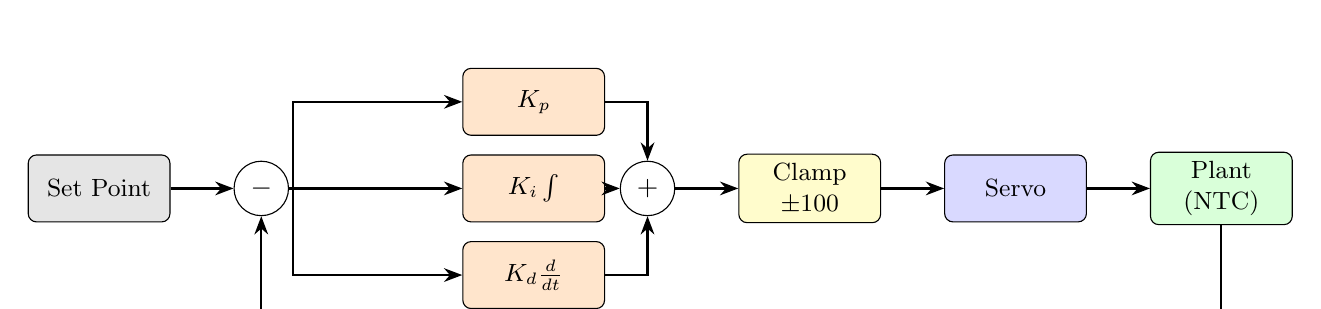
\begin{tikzpicture}[
  block/.style={rectangle, draw, rounded corners=3pt, minimum width=1.8cm, minimum height=0.85cm, align=center, font=\small},
  arr/.style={-Stealth, thick},
  node distance=0.8cm
]
  \node[block, fill=gray!20] (sp) {Set Point};
  \node[circle, draw, right=of sp, minimum size=0.65cm] (sum) {$-$};
  \node[block, fill=orange!20, right=2.2cm of sum, yshift=1.1cm] (kp)  {$K_p$};
  \node[block, fill=orange!20, right=2.2cm of sum]                (ki) {$K_i \int$};
  \node[block, fill=orange!20, right=2.2cm of sum, yshift=-1.1cm] (kd)  {$K_d \frac{d}{dt}$};
  \node[circle, draw, right=4.2cm of sum, minimum size=0.65cm] (sum2) {$+$};
  \node[block, fill=yellow!20, right=of sum2] (sat) {Clamp\\$\pm 100$};
  \node[block, fill=blue!15, right=of sat] (act)  {Servo};
  \node[block, fill=green!15, right=of act] (plant) {Plant\\(NTC)};

  \draw[arr] (sp) -- (sum);
  \draw[arr] (sum) -- ++(0.4,0) |- (kp);
  \draw[arr] (sum) -- ++(0.4,0) |- (ki);
  \draw[arr] (sum) -- ++(0.4,0) |- (kd);
  \draw[arr] (kp) -| (sum2);
  \draw[arr] (ki) -- (sum2);
  \draw[arr] (kd) -| (sum2);
  \draw[arr] (sum2) -- (sat);
  \draw[arr] (sat) -- (act);
  \draw[arr] (act) -- (plant);
  \draw[arr] (plant.south) |- ++(0,-1.2) -| (sum.south);
\end{tikzpicture}
\caption{PID block diagram: three parallel paths sum into a clamped output that drives the servo.}
\label{fig:pid_block}
\end{figure}

\subsection{Tuning Recipe}

The lab brief recommends an empirical PID-tuning procedure \cite{labbrief}:
\begin{enumerate}
  \item Set the desired SP and initialise $K_p = K_i = K_d = 0$.
  \item Increase $K_p$ until the response begins to oscillate, then halve it.
  \item Slowly increase $K_d$ to attenuate the residual oscillations.
  \item Slowly increase $K_i$ until the steady-state error vanishes; reduce by half if oscillation re-appears.
  \item Test under multiple set-point steps; verify the response stays stable and fast.
\end{enumerate}
The interactive serial commands \texttt{P}, \texttt{I}, \texttt{D}, and \texttt{RESET} make this procedure practical without recompiling.

\subsection{Q8.8 Fixed-Point on AVR}

The ATmega2560 has no FPU, so floating-point arithmetic is emulated in software at considerable cost. A \emph{Q8.8 fixed-point} representation keeps the gains in \texttt{int32\_t} as $g \cdot 256$: the upper 24 bits hold the integer part, the lower 8 bits hold $1/256$ fractional units.

\begin{figure}[H]
\centering
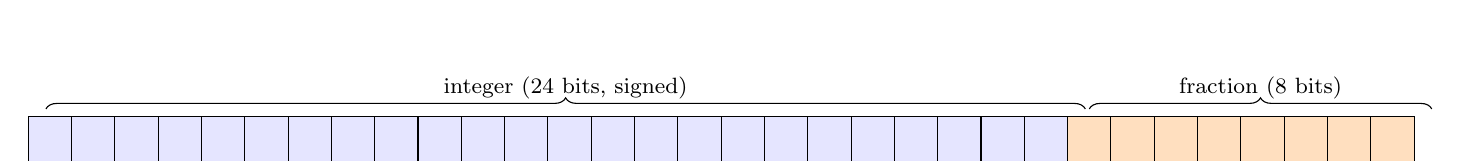
\begin{tikzpicture}[
  bit/.style={rectangle, draw, minimum width=0.55cm, minimum height=0.7cm, font=\tiny}
]
  \foreach \i in {0,...,23} \node[bit, fill=blue!10] at (\i*0.55, 0) {};
  \foreach \i in {24,...,31} \node[bit, fill=orange!25] at (\i*0.55, 0) {};
  \draw[decorate, decoration={brace, amplitude=4pt}] (-0.05,0.45) -- (24*0.55-0.05,0.45) node[midway, above, font=\footnotesize]{integer (24 bits, signed)};
  \draw[decorate, decoration={brace, amplitude=4pt}] (24*0.55,0.45) -- (32*0.55-0.05,0.45) node[midway, above, font=\footnotesize]{fraction (8 bits)};
\end{tikzpicture}
\caption{Q8.8 fixed-point layout (\texttt{int32\_t}). Multiplication of a Q8.8 by an \texttt{int16\_t} yields a Q8.8 result; right-shifting by 8 strips the fractional bits.}
\label{fig:q88}
\end{figure}

The arithmetic identities used in the PID step are:
\begin{align}
g_{Q8.8} &= \mathrm{round}(g \cdot 256) \\
g \cdot x &= (g_{Q8.8} \cdot x) \gg 8 \quad \text{(when $x$ is an integer)}
\end{align}

\subsection{Technology Stack}

\begin{table}[H]
\centering
\begin{tabular}{@{}lll@{}}
\toprule
\textbf{Layer} & \textbf{Technology} & \textbf{Details} \\
\midrule
Hardware Platform    & Arduino Mega 2560  & ATmega2560, 16\,MHz \\
Build System         & PlatformIO         & \texttt{atmelavr}, Arduino framework \\
RTOS                 & FreeRTOS 10.5.1    & \texttt{feilipu/FreeRTOS} \\
Servo Library        & Arduino Servo 1.3  & \texttt{arduino-libraries/Servo} \\
Sensor               & NTC 10\,k$\Omega$  & $B = 3950$, $R_{fixed} = 10$\,k$\Omega$ \\
Actuator             & Hobby servo        & PWM on D9, range 0--180$^{\circ}$ \\
Operator Interface   & 4$\times$4 keypad  & Rows D2--D5, Cols A1--A4 \\
Numeric Format       & Q8.8 fixed-point   & \texttt{int32\_t} for gains; \texttt{int16\_t} tenths-$^{\circ}$C for PV/SP \\
\bottomrule
\end{tabular}
\caption{Technology Stack}
\label{tab:techstack}
\end{table}

\subsection{System Elements}

\begin{itemize}
  \item \textbf{Arduino Mega 2560 (ATmega2560)}: 256\,KB flash, 8\,KB SRAM, 16\,MHz.
  \item \textbf{NTC Thermistor (A0)}: Same voltage-divider topology as Lab~1.5--1.7.
  \item \textbf{Servo motor (D9)}: Now used as a continuous-position actuator. Centre $90^{\circ}$, full swing $\pm 90^{\circ}$.
  \item \textbf{Keypad 4$\times$4 (D2--D5 / A1--A4)}: Same wiring as Lab~1.7. Columns shifted to A1--A4 because A0 is reserved for the NTC.
  \item \textbf{LEDs}: Green (D12) lights when the regulation error is within $\pm$1.0\,$^{\circ}$C of the set point. Red (D11) lights when the PID output saturates at $\pm 100$. Yellow (D10) toggles every 50\,ms as a heartbeat.
  \item \textbf{PlatformIO}: \texttt{env:mega\_lab10} builds with \texttt{-D USE\_FREERTOS -D ACTIVE\_LAB=10}. \cite{pio}
\end{itemize}

% ─────────────────────────────────────────────────────────────────────────────
\section{Design}
% ─────────────────────────────────────────────────────────────────────────────

\subsection{Architectural Design}

\begin{table}[H]
\centering
\begin{tabular}{@{}p{3.6cm}p{2.8cm}p{6.0cm}@{}}
\toprule
\textbf{Component} & \textbf{Role} & \textbf{Interface / Key Operation} \\
\midrule
NTC Thermistor (A0) & Analog input    & Voltage divider \\
NtcSensor          & Sensor driver   & \texttt{ReadNtcRaw}, \texttt{NtcAdcToTempC10} \\
Servo (D9)         & Actuator driver & \texttt{Servo::write} \\
LedDriver          & GPIO output     & \texttt{InitializeLed}, \texttt{SetLedState} \\
KeypadDriver       & Matrix scanner  & \texttt{ScanKeypad} (debounced) \\
SerialStream       & UART adapter    & \texttt{IStream} over \texttt{HardwareSerial} \\
PidController      & Control alg.    & \texttt{PidStep(...)} (Q8.8 fixed-point) \\
Lab10Config        & Configuration   & Pins, gains, intervals, anti-windup limits \\
Lab10Sync          & Shared state    & \texttt{volatile} variables + mutex \\
TaskAcquisition10  & Sensor task     & 50\,ms ADC read \\
TaskCommandRead10  & Operator task   & 50\,ms serial + keypad parser; tuning commands \\
TaskControl10      & Control task    & 100\,ms PID step \\
TaskActuator10     & Actuator task   & 50\,ms servo + LED update \\
TaskDisplay10      & Reporting task  & 500\,ms Plotter + status line \\
MainLab10          & Entry point     & Creates mutex + 5 tasks; starts scheduler \\
\bottomrule
\end{tabular}
\caption{Software Component Roles}
\label{tab:components}
\end{table}

\subsection{Layered Software Architecture}

\begin{figure}[H]
\centering
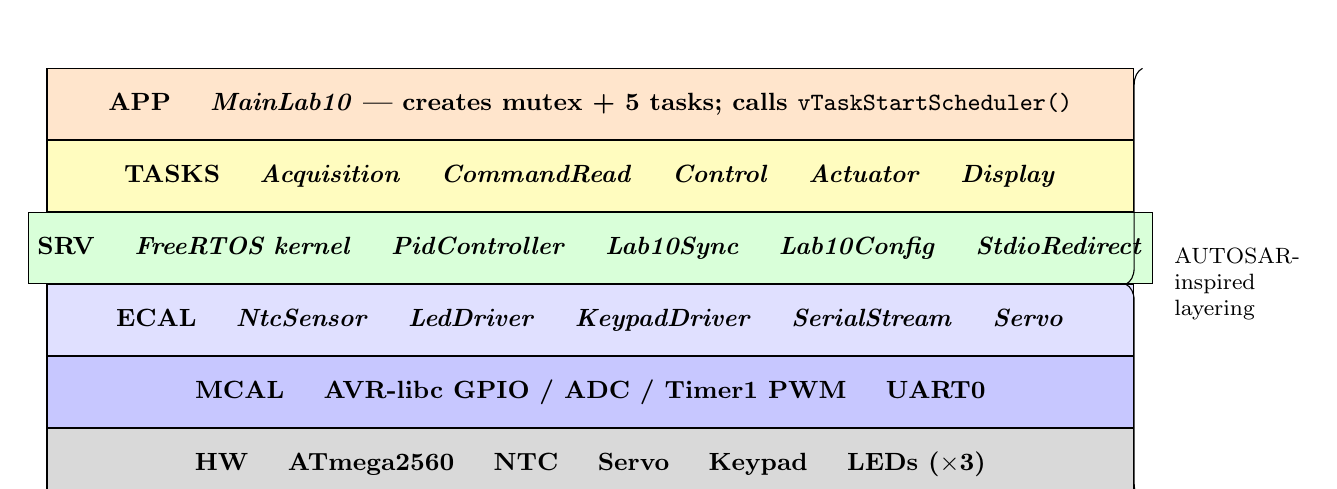
\begin{tikzpicture}[node distance=0pt]
  \def\LW{13.8cm}
  \node[layer, minimum width=\LW, fill=orange!20] (app)
    {\textbf{APP} \quad \textit{MainLab10} --- creates mutex + 5 tasks; calls \texttt{vTaskStartScheduler()}};
  \node[layer, minimum width=\LW, fill=yellow!25, below=of app] (tasks)
    {\textbf{TASKS} \quad \textit{Acquisition} \quad \textit{CommandRead} \quad \textit{Control} \quad \textit{Actuator} \quad \textit{Display}};
  \node[layer, minimum width=\LW, fill=green!15, below=of tasks] (srv)
    {\textbf{SRV} \quad \textit{FreeRTOS kernel} \quad \textit{PidController} \quad \textit{Lab10Sync} \quad \textit{Lab10Config} \quad \textit{StdioRedirect}};
  \node[layer, minimum width=\LW, fill=blue!12, below=of srv] (ecal)
    {\textbf{ECAL} \quad \textit{NtcSensor} \quad \textit{LedDriver} \quad \textit{KeypadDriver} \quad \textit{SerialStream} \quad \textit{Servo}};
  \node[layer, minimum width=\LW, fill=blue!22, below=of ecal] (mcal)
    {\textbf{MCAL} \quad AVR-libc GPIO / ADC / Timer1 PWM \quad UART0};
  \node[layer, minimum width=\LW, fill=gray!30, below=of mcal] (hw)
    {\textbf{HW} \quad ATmega2560 \quad NTC \quad Servo \quad Keypad \quad LEDs ($\times$3)};
  \draw[decorate, decoration={brace, amplitude=6pt, mirror}]
    ([xshift=3pt]app.north east) -- ([xshift=3pt]hw.south east)
    node[midway, right=8pt, font=\footnotesize, align=left]
    {AUTOSAR-\\inspired\\layering};
\end{tikzpicture}
\caption{Layered Software Architecture}
\label{fig:layers}
\end{figure}

\subsection{One PID Control Tick --- Sequence Diagram}

\begin{figure}[H]
\centering
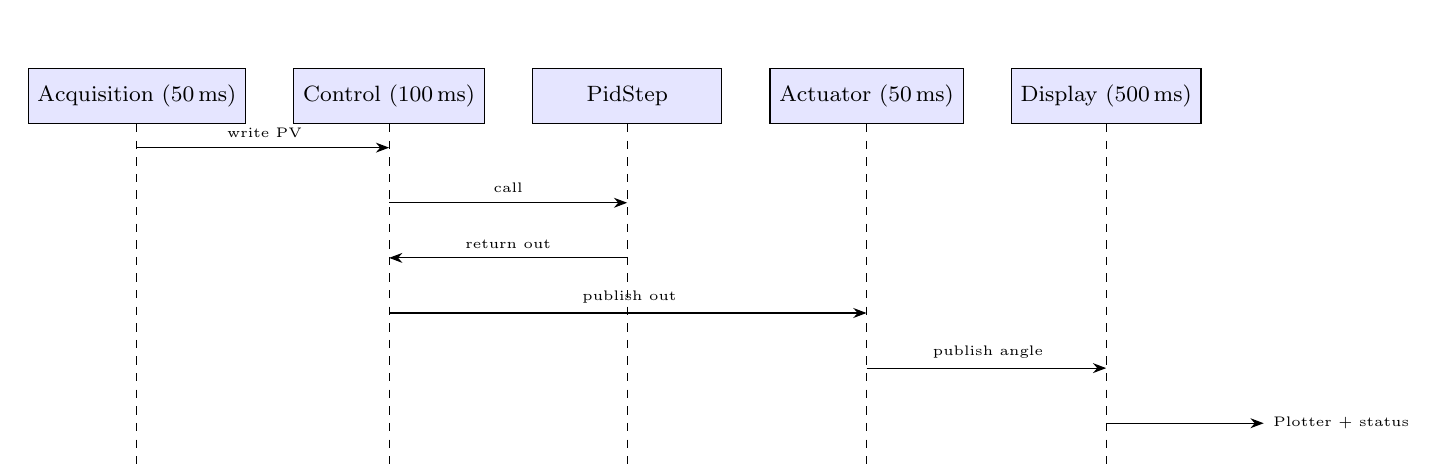
\begin{tikzpicture}[
  ent/.style={rectangle, draw, fill=blue!10, minimum width=2.4cm, minimum height=0.7cm, font=\footnotesize},
  arr/.style={-Stealth},
  msg/.style={font=\tiny},
  node distance=0.6cm
]
  \node[ent] (acq)   {Acquisition (50\,ms)};
  \node[ent, right=of acq] (ctrl)  {Control (100\,ms)};
  \node[ent, right=of ctrl] (pid) {PidStep};
  \node[ent, right=of pid]  (act)  {Actuator (50\,ms)};
  \node[ent, right=of act]  (disp) {Display (500\,ms)};

  \foreach \n in {acq, ctrl, pid, act, disp}
    \draw[dashed] (\n.south) -- ++(0,-4.5);

  \draw[arr] ($(acq.south) + (0,-0.3)$)  -- node[msg, above]{\,write PV} ($(ctrl.south) + (0,-0.3)$);
  \draw[arr] ($(ctrl.south) + (0,-1.0)$) -- node[msg, above]{call} ($(pid.south)  + (0,-1.0)$);
  \draw[arr] ($(pid.south)  + (0,-1.7)$) -- node[msg, above]{return out} ($(ctrl.south) + (0,-1.7)$);
  \draw[arr] ($(ctrl.south) + (0,-2.4)$) -- node[msg, above]{\,publish out} ($(act.south)  + (0,-2.4)$);
  \draw[arr] ($(act.south)  + (0,-3.1)$) -- node[msg, above]{\,publish angle} ($(disp.south) + (0,-3.1)$);
  \draw[arr] ($(disp.south) + (0,-3.8)$) -- ++(2.0, 0) node[right, msg]{Plotter + status};
\end{tikzpicture}
\caption{One full PID control tick across the five tasks.}
\label{fig:seq}
\end{figure}

\subsection{Output Mapping to Servo Angle}

The PID output is a signed integer in $[-100, +100]$. The servo angle is centred at $90^{\circ}$ and swings $\pm 90^{\circ}$:
\begin{equation}
\text{angle} = 90 + \left\lfloor \frac{\mathrm{out} \cdot 90}{100} \right\rfloor, \quad
\text{angle} \in [0^{\circ}, 180^{\circ}]
\label{eq:servo_map}
\end{equation}
This produces an actuation that is symmetric around the neutral position: positive outputs (PV below SP) tilt the servo towards \enquote{heat}, negative outputs tilt towards \enquote{cool}.

\subsection{LED Status Logic}

\begin{itemize}
  \item \textbf{Green (D12)}: ON when $|e| \le 10$ tenths-$^{\circ}$C ($\equiv$ within $\pm 1.0\,^{\circ}$C of SP). Indicates the system is in-band.
  \item \textbf{Red (D11)}: ON when $|\mathrm{out}| = 100$. Indicates the PID has saturated; if it stays lit for long, raise gains or check actuator authority.
  \item \textbf{Yellow (D10)}: Toggles each Actuator tick (50\,ms) as a heartbeat.
\end{itemize}

\subsection{Electronic Design}

\begin{figure}[H]
\centering
\begin{tikzpicture}[
  blk/.style={rectangle, draw, minimum height=1.4cm, align=center, font=\small},
  mcu/.style={blk, fill=gray!15, minimum width=3.0cm, minimum height=8.5cm},
  sens/.style={blk, fill=orange!20, minimum width=2.0cm, minimum height=0.75cm},
  ledg/.style={blk, fill=green!20, minimum width=2.0cm, minimum height=0.75cm},
  ledr/.style={blk, fill=red!20,   minimum width=2.0cm, minimum height=0.75cm},
  ledy/.style={blk, fill=yellow!30, minimum width=2.0cm, minimum height=0.75cm},
  act/.style ={blk, fill=blue!20, minimum width=2.0cm, minimum height=0.75cm},
  bus/.style={-Stealth, thick},
  lbl/.style={font=\tiny, midway},
]
  \node[mcu] (mcu) {Arduino Mega\\2560\\[4pt]
    \tiny A0 $\leftarrow$ NTC\\
    A1--A4 $\leftarrow$ Keypad cols\\
    D2--D5 $\to$ Keypad rows\\
    D9 $\to$ Servo PWM\\
    D10 $\to$ Yellow LED\\
    D11 $\to$ Red LED\\
    D12 $\to$ Green LED\\
    UART0 TX/RX};

  \node[sens, left=2.6cm of mcu, yshift=2.8cm] (ntc) {NTC\\{\tiny A0, 10\,k$\Omega$ divider}};
  \node[blk, fill=gray!20, left=2.6cm of mcu, yshift=0cm, minimum width=2.0cm, minimum height=1.6cm] (kp) {Keypad 4$\times$4\\{\tiny rows D2--D5\\cols A1--A4}};

  \node[act, right=2.6cm of mcu, yshift=2.8cm] (servo) {Servo\\{\tiny D9, PWM}};
  \node[ledg, right=2.6cm of mcu, yshift=1.4cm] (gled) {Green LED\\{\tiny D12, 220\,$\Omega$}};
  \node[ledr, right=2.6cm of mcu, yshift=0.4cm] (rled) {Red LED\\{\tiny D11, 220\,$\Omega$}};
  \node[ledy, right=2.6cm of mcu, yshift=-0.6cm] (yled) {Yellow LED\\{\tiny D10, 220\,$\Omega$}};
  \node[blk, fill=blue!10, right=2.6cm of mcu, yshift=-2.0cm, minimum width=2.0cm, minimum height=0.75cm] (ser) {PC Terminal\\{\tiny UART 9600 baud}};

  \draw[bus] (ntc.east) -- node[lbl, above]{A0} (mcu.west |- ntc.east);
  \draw[bus, Stealth-Stealth] (kp.east) -- node[lbl, above]{8 pins} (mcu.west |- kp.east);
  \draw[bus] (mcu.east |- servo.west) -- node[lbl, above]{D9} (servo.west);
  \draw[bus] (mcu.east |- gled.west)  -- node[lbl, above]{D12} (gled.west);
  \draw[bus] (mcu.east |- rled.west)  -- node[lbl, above]{D11} (rled.west);
  \draw[bus] (mcu.east |- yled.west)  -- node[lbl, above]{D10} (yled.west);
  \draw[bus, Stealth-Stealth] (mcu.east |- ser.west) --
    node[lbl, above]{TX/RX} (ser.west);
\end{tikzpicture}
\caption{Electronic Design --- Pin Connection Diagram (identical to Lab~1.7)}
\label{fig:elec}
\end{figure}

% ─────────────────────────────────────────────────────────────────────────────
\section{Implementation}
% ─────────────────────────────────────────────────────────────────────────────

\subsection{Project Structure}

\begin{table}[H]
\centering
\begin{tabular}{@{}lp{8.0cm}@{}}
\toprule
\textbf{File} & \textbf{Purpose} \\
\midrule
\texttt{src/main.cpp}                        & Lab dispatcher \\
\texttt{src/labs/lab10/MainLab10.cpp}        & Defines shared state; creates mutex + 5 tasks; starts scheduler \\
\texttt{src/labs/lab10/TaskAcquisition10.cpp}& 50\,ms NTC sample $\to$ tenths $^{\circ}$C \\
\texttt{src/labs/lab10/TaskCommandRead10.cpp}& 50\,ms serial + keypad parser; \texttt{P/I/D/RESET} dispatch \\
\texttt{src/labs/lab10/TaskControl10.cpp}    & 100\,ms PID step \\
\texttt{src/labs/lab10/TaskActuator10.cpp}   & 50\,ms output $\to$ servo angle; LEDs \\
\texttt{src/labs/lab10/TaskDisplay10.cpp}    & 500\,ms Plotter + status with current gains \\
\texttt{src/labs/lab10/PidController.cpp}    & Q8.8 PID step (anti-windup + output clamp) \\
\texttt{include/labs/lab10/Lab10Config.h}    & Pins, intervals, default gains, limits \\
\texttt{include/labs/lab10/Lab10Sync.h}      & Shared volatile + mutex \\
\texttt{include/labs/lab10/PidController.h}  & \texttt{PidStep} signature \\
\bottomrule
\end{tabular}
\caption{Project File Structure}
\label{tab:files}
\end{table}

\subsection{PlatformIO Environment Configuration}

\begin{lstlisting}
[env:mega_lab10]
extends = env:mega
lib_deps =
    ${env:mega.lib_deps}
    arduino-libraries/Servo@^1.3.0
    feilipu/FreeRTOS@^10.5.1-1
    fmalpartida/LiquidCrystal@^1.5.0
build_flags =
    -Wno-error=unused-variable
    -D F_CPU=16000000L
    -D USE_FREERTOS
    -D ACTIVE_LAB=10
\end{lstlisting}

\subsection{Configuration Constants}

\begin{lstlisting}[caption={Lab10Config.h --- key constants}]
const uint8_t  NtcAnalogPin10        = A0;
const uint8_t  ServoPin10            = 9;
const uint8_t  GreenLedPin10         = 12;
const uint8_t  RedLedPin10           = 11;
const uint8_t  YellowLedPin10        = 10;

const int16_t  SetPointDefaultC10_10 = 250;  // 25.0 C
const int16_t  SetPointMinC10_10     = -100;
const int16_t  SetPointMaxC10_10     = 500;

// PID gains (Q8.8 fixed-point: stored * 256). Defaults Kp=4.0 Ki=0.10 Kd=0.50.
const int32_t  Kp_Q88_Default = (int32_t)(4.0f  * 256);  // = 1024
const int32_t  Ki_Q88_Default = (int32_t)(0.10f * 256);  // =   26
const int32_t  Kd_Q88_Default = (int32_t)(0.50f * 256);  // =  128

const int16_t  OutputMax10        = 100;
const uint8_t  ServoCenterAngle10 = 90;
const uint8_t  ServoSwingAngle10  = 90;
const int32_t  IntegralLimit10    = 5000;   // anti-windup clamp

const uint16_t AcquisitionIntervalMs10 = 50;
const uint16_t ControlIntervalMs10     = 100; // PID period
const uint16_t ActuatorIntervalMs10    = 50;
const uint16_t CommandIntervalMs10     = 50;
const uint16_t DisplayIntervalMs10     = 500;
\end{lstlisting}

\subsection{Shared State and Synchronisation}

\begin{lstlisting}[caption={Lab10Sync.h --- shared volatile data and mutex}]
extern volatile uint16_t Lab10RawAdc;
extern volatile int16_t  Lab10TempC10;       // PV
extern volatile int16_t  Lab10SetPointC10;   // SP
extern volatile int32_t  Lab10KpQ88;         // PID gains, Q8.8
extern volatile int32_t  Lab10KiQ88;
extern volatile int32_t  Lab10KdQ88;
extern volatile int32_t  Lab10Integral;      // PID internal state
extern volatile int16_t  Lab10PrevError;
extern volatile int16_t  Lab10Output;        // clamped [-100, +100]
extern volatile uint8_t  Lab10ServoAngle;

extern SemaphoreHandle_t xLab10Mutex;
\end{lstlisting}

\subsection{PidController Module}

The PID step lives in its own translation unit and contains no Arduino dependencies, making it trivially unit-testable. Inputs are passed in tenths-$^{\circ}$C and Q8.8 gains; \texttt{integral} and \texttt{prevError} are owned by the caller (so two independent PID loops can coexist).

\begin{lstlisting}[caption={PidController.cpp --- the full PID step}]
int16_t PidStep(int16_t setPoint, int16_t measured,
                int32_t kpQ88, int32_t kiQ88, int32_t kdQ88,
                int32_t* integral, int16_t* prevError,
                int32_t integralLimit, int16_t outputMax) {
    int16_t error = (int16_t)(setPoint - measured);

    // Integral with anti-windup clamp.
    int32_t newIntegral = *integral + error;
    if (newIntegral >  integralLimit) newIntegral =  integralLimit;
    if (newIntegral < -integralLimit) newIntegral = -integralLimit;
    *integral = newIntegral;

    // Discrete derivative.
    int16_t derivative = (int16_t)(error - *prevError);
    *prevError = error;

    // Sum of three contributions in Q8.8.
    int32_t outQ88 = kpQ88 * (int32_t)error
                   + kiQ88 * newIntegral
                   + kdQ88 * (int32_t)derivative;

    int32_t out = outQ88 >> 8;          // strip Q8.8 fractional bits
    if (out >  outputMax) out =  outputMax;
    if (out < -outputMax) out = -outputMax;
    return (int16_t)out;
}
\end{lstlisting}

A few implementation notes:
\begin{itemize}
  \item \textbf{Integer-only arithmetic}: every operation is on \texttt{int16\_t} or \texttt{int32\_t}; no floating-point is invoked.
  \item \textbf{Anti-windup}: \texttt{integralLimit = 5000} is applied \emph{before} the integral is fed into the multiplication, preventing the accumulator from drifting unboundedly during long actuator saturation.
  \item \textbf{Output clamp}: $\pm$\texttt{outputMax} = $\pm 100$, matching the actuator mapping in Equation~\ref{eq:servo_map}.
  \item \textbf{Caller owns state}: \texttt{integral} and \texttt{prevError} are pointers to the task's storage, so the function itself is stateless.
\end{itemize}

\subsection{TaskControl10 --- 100\,ms PID Tick}

\begin{lstlisting}[caption={TaskControl10 --- mutex-protected PID step}]
void TaskControl10Func(void* pv) {
    const TickType_t Interval = pdMS_TO_TICKS(ControlIntervalMs10);
    TickType_t xLastWakeTime = xTaskGetTickCount();
    for (;;) {
        xSemaphoreTake(xLab10Mutex, portMAX_DELAY);
        int16_t pv      = Lab10TempC10;
        int16_t sp      = Lab10SetPointC10;
        int32_t kp      = Lab10KpQ88;
        int32_t ki      = Lab10KiQ88;
        int32_t kd      = Lab10KdQ88;
        int32_t integ   = Lab10Integral;
        int16_t prevErr = Lab10PrevError;
        xSemaphoreGive(xLab10Mutex);

        int16_t output = PidStep(sp, pv, kp, ki, kd,
                                 &integ, &prevErr,
                                 IntegralLimit10, OutputMax10);

        xSemaphoreTake(xLab10Mutex, portMAX_DELAY);
        Lab10Integral  = integ;
        Lab10PrevError = prevErr;
        Lab10Output    = output;
        xSemaphoreGive(xLab10Mutex);
        vTaskDelayUntil(&xLastWakeTime, Interval);
    }
}
\end{lstlisting}

The 100\,ms period is intentionally slower than the 50\,ms acquisition tick: PID needs samples \emph{far enough apart} for the discrete derivative to be meaningful in the presence of ADC noise.

\subsection{TaskActuator10 --- Servo Mapping and LEDs}

\begin{lstlisting}[caption={TaskActuator10 --- output $\to$ servo angle, LEDs}]
int16_t scaled = (int16_t)((int32_t)out * ServoSwingAngle10 / OutputMax10);
int16_t angle  = (int16_t)ServoCenterAngle10 + scaled;
if (angle < 0)   angle = 0;
if (angle > 180) angle = 180;
Lab10Servo.write((uint8_t)angle);

// Status LEDs
bool saturated = (out >= OutputMax10) || (out <= -OutputMax10);
bool inBand    = (sp - pv >= -10 && sp - pv <= 10);
SetLedState(GreenLedPin10, inBand);
SetLedState(RedLedPin10,   saturated);
yellowBlink = !yellowBlink;
SetLedState(YellowLedPin10, yellowBlink);
\end{lstlisting}

\subsection{TaskCommandRead10 --- Tuning Commands}

The command parser handles both numeric set-point entry (via serial line and keypad) and the tuning commands. The Q8.8 parser is small enough to fit inline:

\begin{lstlisting}[caption={ParseQ88 --- decimal string $\to$ Q8.8 fixed-point}]
static bool ParseQ88(const char* s, int32_t* outQ88) {
    int sign = 1;
    if (*s == '-') { sign = -1; ++s; } else if (*s == '+') ++s;
    int32_t intPart = 0;
    bool sawDigit = false;
    while (*s >= '0' && *s <= '9') {
        intPart = intPart * 10 + (*s - '0');
        sawDigit = true; ++s;
    }
    int32_t fracNum = 0, fracDen = 1;
    if (*s == '.') {
        ++s;
        for (uint8_t i = 0; i < 4 && *s >= '0' && *s <= '9'; ++i) {
            fracNum = fracNum * 10 + (*s - '0');
            fracDen *= 10; sawDigit = true; ++s;
        }
    }
    if (!sawDigit || *s != '\0') return false;
    int32_t q88 = intPart * 256 + (fracNum * 256 + fracDen / 2) / fracDen;
    *outQ88 = sign * q88;
    return true;
}
\end{lstlisting}

\begin{lstlisting}[caption={ProcessSerialLine --- P/I/D/RESET dispatch}]
char head = (char)toupper((unsigned char)*line);
if (head == 'P' || head == 'I' || head == 'D') {
    int32_t q88;
    if (!ParseQ88(arg, &q88)) { printf_P(PSTR("[bad gain]\n")); return; }
    xSemaphoreTake(xLab10Mutex, portMAX_DELAY);
    if      (head == 'P') Lab10KpQ88 = q88;
    else if (head == 'I') Lab10KiQ88 = q88;
    else                  Lab10KdQ88 = q88;
    Lab10Integral = 0; Lab10PrevError = 0;   // avoid windup kick
    xSemaphoreGive(xLab10Mutex);
    return;
}
if (head == 'R') {              // "RESET"
    xSemaphoreTake(xLab10Mutex, portMAX_DELAY);
    Lab10Integral = 0; Lab10PrevError = 0; Lab10Output = 0;
    xSemaphoreGive(xLab10Mutex);
    return;
}
// Plain integer -> setpoint in whole degrees C
long value = strtol(line, &endPtr, 10);
if (endPtr != line) SubmitSetPoint10((int16_t)(value * 10));
\end{lstlisting}

Resetting the integrator on every gain change is critical: without it, switching from \texttt{Kp=4.0} to \texttt{Kp=0.5} while the integral has accumulated would suddenly cause a giant kick when the new $K_i$ multiplies a stale integrator. Better to start fresh.

\subsection{TaskDisplay10 --- Plotter and Status with Gains}

\begin{lstlisting}[caption={TaskDisplay10 --- 500\,ms output with Q8.8 gain decode}]
printf_P(PSTR("SP:%d\tPV:%d\tOUT:%d\tANG:%u\n"), sp, pv, out, angle);

long kpx = (long)kpQ88 * 10000 / 256;
long kix = (long)kiQ88 * 10000 / 256;
long kdx = (long)kdQ88 * 10000 / 256;
printf_P(PSTR("# SP=%d.%d C  PV=%d.%d C  OUT=%d  Kp=%ld.%04ld Ki=%ld.%04ld Kd=%ld.%04ld\n"),
    sp/10, abs(sp)%10, pv/10, abs(pv)%10, out,
    kpx/10000, labs(kpx)%10000,
    kix/10000, labs(kix)%10000,
    kdx/10000, labs(kdx)%10000);
\end{lstlisting}

The \texttt{kpx = (long)kpQ88 * 10000 / 256} expression converts Q8.8 to 4-decimal-digit integer scaling: a stored \texttt{Kp = 1024} (= 4.0 in Q8.8) prints as \texttt{4.0000}. The display thus reflects the exact gain applied by the controller.

\subsection{Setup and Scheduler Launch}

\begin{lstlisting}[caption={SetupLab10 --- task creation and welcome banner}]
void SetupLab10() {
    SerialIo.begin(9600);
    initStdio(&SerialIo);
    InitializeNtcSensor(NtcAnalogPin10);
    InitializeLed(GreenLedPin10);
    InitializeLed(RedLedPin10);
    InitializeLed(YellowLedPin10);
    InitializeKeypad(RowPins, ColPins);
    xLab10Mutex = xSemaphoreCreateMutex();

    xTaskCreate(TaskAcquisition10Func, "Acq",  192, nullptr, 3, nullptr);
    xTaskCreate(TaskCommandRead10Func, "Cmd",  256, nullptr, 3, nullptr);
    xTaskCreate(TaskControl10Func,     "PID",  192, nullptr, 2, nullptr);
    xTaskCreate(TaskActuator10Func,    "Act",  192, nullptr, 2, nullptr);
    xTaskCreate(TaskDisplay10Func,     "Disp", 256, nullptr, 1, nullptr);

    printf_P(PSTR("Lab 10: PID Control (Variant D - servo)\n"));
    printf_P(PSTR("Tune via serial: 'P1.5'  'I0.05'  'D0.5'  'RESET'\n"));
    vTaskStartScheduler();
}
\end{lstlisting}

\subsection{STDIO Usage}

\begin{table}[H]
\centering
\begin{tabular}{@{}lp{4cm}p{6.0cm}@{}}
\toprule
\textbf{Function} & \textbf{Call site} & \textbf{Output} \\
\midrule
\texttt{printf\_P} & \texttt{SetupLab10} (5$\times$) & Welcome banner; default SP, PID period; tuning help \\
\texttt{printf\_P} & \texttt{TaskCommandRead10}      & \texttt{[SP=...]}, \texttt{[P=4.0000]}, \texttt{[PID reset]}, \texttt{[bad gain ...]} \\
\texttt{printf\_P} & \texttt{TaskDisplay10} (2$\times$) & Plotter line + human-readable status with current gains \\
\bottomrule
\end{tabular}
\caption{STDIO Usage}
\label{tab:stdio}
\end{table}

\subsection{Code}

The complete source is available at the GitHub repository listed as the first entry in the bibliography \cite{code}.

% ─────────────────────────────────────────────────────────────────────────────
\section{Results}\label{sec:results}
% ─────────────────────────────────────────────────────────────────────────────

The application was verified on physical hardware and observed via the Arduino Serial Plotter. The following scenarios were tested:
\begin{enumerate}
  \item \textbf{Default convergence}: With $K_p$=4.0, $K_i$=0.10, $K_d$=0.50 and SP=25.0\,$^{\circ}$C the PV converges to within $\pm 0.2\,^{\circ}$C of the set point and stays there; the green LED is on.
  \item \textbf{Step response}: Changing SP from 25 to 30\,$^{\circ}$C (\texttt{30 + Enter}) produces a smooth rise without hard overshoot; the red LED briefly lights as the output saturates at +100 during the transient.
  \item \textbf{Pure proportional}: \texttt{I0}, \texttt{D0}, \texttt{P2.0} reveals the steady-state offset characteristic of P-only control.
  \item \textbf{PI tuning}: Adding \texttt{I0.05} eliminates the offset within $\sim$30\,s.
  \item \textbf{PID damping}: Adding \texttt{D0.5} reduces the overshoot of the step response.
  \item \textbf{Reset}: \texttt{RESET} clears integral and previous-error in one command, useful when re-tuning.
  \item \textbf{Anti-windup}: Forcing a large step (SP=50, room temperature 23) saturates the output at +100; on returning to 25\,$^{\circ}$C the system does not overshoot wildly because the integral was clamped to $\pm$5000.
  \item \textbf{Bad gain rejection}: \texttt{P abc} prints \texttt{[bad gain: P abc]} without affecting state.
  \item \textbf{Display gains}: The 500\,ms status line always shows the currently active gains; switching from \texttt{P4.0} to \texttt{P2.0} is reflected on the next tick.
  \item \textbf{Yellow heartbeat}: The yellow LED toggles every 50\,ms.
\end{enumerate}

A sample serial monitor output:

\begin{lstlisting}
Lab 10: PID Control (Variant D - servo)
Sensor: NTC on A0  Servo: D9
SP=25.0 C  PID period=100 ms
Setpoint: serial 'NN' or keypad NN '#'  *=clr A/B=+/-1 C/D=+/-10
Tune via serial: 'P1.5'  'I0.05'  'D0.5'  'RESET'
SP:250  PV:243  OUT:30   ANG:117
# SP=25.0 C  PV=24.3 C  OUT=30  Kp=4.0000 Ki=0.1015 Kd=0.5000
SP:250  PV:248  OUT:12   ANG:100
# SP=25.0 C  PV=24.8 C  OUT=12  Kp=4.0000 Ki=0.1015 Kd=0.5000
[SP=30.0 C]
SP:300  PV:251  OUT:100  ANG:180
# SP=30.0 C  PV=25.1 C  OUT=100 Kp=4.0000 Ki=0.1015 Kd=0.5000
[P=2.0000]
SP:300  PV:281  OUT:62   ANG:145
# SP=30.0 C  PV=28.1 C  OUT=62  Kp=2.0000 Ki=0.1015 Kd=0.5000
[PID reset]
\end{lstlisting}

\subsection{Test Validation}

\begin{table}[H]
\centering
\begin{tabular}{@{}llp{7.5cm}@{}}
\toprule
\textbf{Test ID} & \textbf{Result} & \textbf{Observations} \\
\midrule
RF01\_T01  & Pass & Acquisition reads NTC every 50\,ms; PV stored as tenths $^{\circ}$C. \\
RF02\_T01  & Pass & PID converges to SP under default gains ($K_p$=4.0, $K_i$=0.10, $K_d$=0.50). \\
RF03\_T01  & Pass & Step response (25 $\to$ 30\,$^{\circ}$C) settles within $\pm$0.2\,$^{\circ}$C and no sustained overshoot. \\
RF04\_T01  & Pass & P-only control exhibits steady-state offset; adding \texttt{I0.05} eliminates it. \\
RF05\_T01  & Pass & Adding $K_d$ damps the transient; smaller overshoot, faster settling. \\
RF06\_T01  & Pass & Output mapping $90 + \mathrm{out} \cdot 90/100$ is symmetric and clipped to [0, 180]. \\
RF07\_T01  & Pass & Anti-windup clamp ($\pm$5000) prevents integral runaway during saturation. \\
RF08\_T01  & Pass & \texttt{P/I/D <float>} updates the corresponding gain and resets integrator. \\
RF09\_T01  & Pass & \texttt{RESET} clears integral, previous error, and output. \\
RF10\_T01  & Pass & Display task prints Plotter line + human-readable status with current gains every 500\,ms. \\
RF11\_T01  & Pass & Green LED tracks $|e| \le 1$\,$^{\circ}$C; red LED tracks $|\mathrm{out}|=100$. \\
RNF01\_T01 & Pass & Five tasks run concurrently; no deadlock or data corruption observed. \\
RNF02\_T01 & Pass & PidController is a separate, dependency-free translation unit. \\
RNF03\_T01 & Pass & All PID arithmetic uses Q8.8 fixed-point; no \texttt{float} appears in the hot path. \\
RNF04\_T01 & Pass & Single \texttt{xLab10Mutex} protects every shared volatile variable. \\
RNF05\_T01 & Pass & Pin numbers, intervals, gains, and limits are all named constants. \\
RNF06\_T01 & Pass & Bad gain strings are rejected; firmware state is unaffected. \\
RNF07\_T01 & Pass & PROGMEM strings (\texttt{printf\_P}) keep SRAM usage low. \\
\bottomrule
\end{tabular}
\caption{Test Results for the PID Control Application}
\label{tab:tests}
\end{table}

% ─────────────────────────────────────────────────────────────────────────────
\section{Note on AI}
% ─────────────────────────────────────────────────────────────────────────────

\hspace{0.8cm}
For this laboratory work, AI assistants such as Claude~4.7~Opus were used for explaining the theoretical background of PID control, suggesting how to formulate the discrete update step, recommending Q8.8 fixed-point as a way to avoid the AVR floating-point cost, and for paraphrasing and structuring ideas in this report. All AI-generated content was reviewed against the implementation and against authoritative references (Åström \& Hägglund \cite{astrom}). The PID gains were tuned empirically on the simulated and physical plant.

% ─────────────────────────────────────────────────────────────────────────────
\section{Conclusion}
% ─────────────────────────────────────────────────────────────────────────────

\hspace{0.8cm}
This laboratory work demonstrated automatic temperature control with a Proportional--Integral--Derivative regulator on an ATmega2560 running FreeRTOS. The same plant and hardware as Lab~1.7 (NTC on A0, servo on D9) were reused with no electrical modification; only the control law and the actuator mapping changed. The PID step is a small, dependency-free function operating on Q8.8 fixed-point gains and tenths-$^{\circ}$C integers --- no floating-point appears in the hot path, which keeps the controller fast and its timing deterministic on a CPU without an FPU.

\hspace{0.8cm}
Five FreeRTOS tasks (Acquisition 50\,ms, CommandRead 50\,ms, Control 100\,ms, Actuator 50\,ms, Display 500\,ms) communicate through shared volatile state under a single mutex, mirroring the architecture of Lab~1.7 but with a slower control period to give the discrete derivative meaningful samples. An anti-windup clamp on the integral, combined with an integrator reset on every gain change, prevents the surprise kicks that plague naive PID implementations.

\hspace{0.8cm}
The serial command interface (\texttt{P}, \texttt{I}, \texttt{D}, \texttt{RESET}, plus numeric set-point) makes the empirical tuning loop fast: a single line in the serial monitor changes a gain at runtime, the new value is echoed back, and the next 500\,ms display tick already shows the controller acting on it. Combined with the Arduino Serial Plotter line, this provides a practical, ergonomic environment for the iterative tuning recipe described in §6.2.2 of the lab brief. The result is a clean closed-loop temperature controller whose behaviour is fully observable, fully tunable, and entirely free of floating-point arithmetic on a microcontroller that has no FPU.

% ─────────────────────────────────────────────────────────────────────────────
\section{Bibliography}
% ─────────────────────────────────────────────────────────────────────────────

\begingroup
\makeatletter
\renewcommand{\section}[2]{}
\makeatother

\begin{thebibliography}{}

  \bibitem{code}
  \url{https://github.com/NeValetik/si-labs}

  \bibitem{labbrief}
  Cojuhari I., Ababii V. \textit{Embedded Systems Laboratory --- Lab~6: Automatic regulation in embedded systems}.
  Technical University of Moldova, 2025.

  \bibitem{astrom}
  Åström K.J., Hägglund T. \textit{PID Controllers: Theory, Design, and Tuning}, 2nd ed.
  Instrument Society of America, 1995.

  \bibitem{q88}
  Wikipedia. \textit{Q (number format)}.
  \url{https://en.wikipedia.org/wiki/Q\_(number\_format)}

  \bibitem{ntc_steinhart}
  Ametherm. \textit{NTC Thermistors --- Steinhart and Hart Equation}.
  \url{https://www.ametherm.com/thermistor/ntc-thermistor-steinhart-hart-equation}

  \bibitem{freertos_mutex}
  FreeRTOS. \textit{Mutexes}.
  \url{https://www.freertos.org/Documentation/02-Kernel/02-Kernel-features/02-Queues-mutexes-and-semaphores/04-Mutexes}

  \bibitem{servo_lib}
  Arduino. \textit{Servo Library Reference}.
  \url{https://www.arduino.cc/reference/en/libraries/servo/}

  \bibitem{pio}
  PlatformIO. \textit{PlatformIO Documentation --- atmelavr Platform}.
  \url{https://docs.platformio.org/en/latest/platforms/atmelavr.html}

  \bibitem{avr}
  Microchip Technology. \textit{ATmega2560 Datasheet}, DS40002211A, 2020.
  \url{https://ww1.microchip.com/downloads/en/devicedoc/atmel-2549-8-bit-avr-microcontroller-atmega640-1280-1281-2560-2561_datasheet.pdf}

\end{thebibliography}
\endgroup

\pagebreak
\end{document}
